\documentclass[conference]{IEEEtran}
\IEEEoverridecommandlockouts
\usepackage{cite}
\usepackage{amsmath,amssymb,amsfonts}
\usepackage{algorithmic}
\usepackage{graphicx}
\usepackage{textcomp}
\usepackage{xcolor}
\usepackage{booktabs}
\usepackage{multirow}
\usepackage{array}
\usepackage{url}
\def\BibTeX{{\rm B\kern-.05em{\sc i\kern-.025em b}\kern-.08em
    T\kern-.1667em\lower.7ex\hbox{E}\kern-.125emX}}

\begin{document}

\title{AdaCraft: Iterative Adaptive Personalization of Educational Examples via Agentic Feedback Loops}

\author{\IEEEauthorblockN{Anonymous Authors}}

\maketitle

\begin{abstract}
Despite growing interest in personalized educational AI, existing systems treat personalization as a static, one-shot operation, where user profiles are read at inference time, a response is generated, and the system cannot adapt when learners signal that their needs were not met \cite{b1, b2}. This static approach misses a fundamental truth about learning: a student's needs change as they interact with content, and a system that cannot respond to that signal is not truly adaptive. We present \textbf{AdaCraft}, an agentic system that generates personalized educational examples through a multi-agent LangGraph workflow and continuously refines them based on natural-language feedback. The system operates through three capability layers: (1) a static user profile capturing demographic and complexity preferences, (2) a Context Manager Agent that retrieves historical learning patterns and synthesizes them into a targeted personalization instruction before each generation, and (3) an Adaptive Response Agent that interprets free-form user feedback and autonomously decides whether to regenerate the example, record a session insight, or persist a new long-term learning pattern. To rigorously measure each layer's contribution, we design a four-tier ablation protocol (T0: generic baseline, T1: +profile, T2: +context manager, T3: full system) grounded in LaMP \cite{b3} and evaluated with a five-axis rubric: Personalization Fidelity, Complexity Calibration, Conceptual Accuracy, Pedagogical Clarity, and Domain Appropriateness, scored by a GPT-4.1-nano primary judge using G-Eval chain-of-thought \cite{b4} and Prometheus 2 rubric injection \cite{b5}, with inter-judge reliability validated against a Llama~3.3~70B secondary judge on a 20\% random subsample. We further introduce three feedback-loop convergence metrics: FCR (Feedback Compliance Rate), LUR (Loop Utilization Rate), and PPU (Pattern Persistence Utilization), to measure the quality of iterative adaptation, not merely its presence. Across two generator configurations (DeepSeek V3.2 and GPT-5-nano), the full system improves over the generic baseline by up to $+1.269$ composite points (DeepSeek: $+0.631$; GPT-5-nano: $+1.269$), with profile injection (T0$\to$T1) as the dominant driver in both runs. The agentic feedback loop proves reliable: FCR@4 $\geq 0.891$ across both providers, loop utilization exceeding 93\%, and stored learning patterns yielding positive PPU deltas ($+0.312$ for DeepSeek, $+1.938$ for GPT-5-nano) for returning users. Inter-judge agreement between the primary GPT-4.1-nano judge and the Llama~3.3~70B secondary judge yielded Cohen's $\kappa \geq 0.607$, confirming cross-provider consistency in the strict four-tier ordering T0 $<$ T1 $<$ T2 $<$ T3. 

%To our knowledge, this is the first evaluation protocol specifically designed for iterative adaptive personalization in educational content generation, a scope distinct from RLHF evaluation, dialogue turn-level evaluation, and iterative text refinement benchmarks, which do not address the joint problem of profile-grounded generation and feedback-driven convergence in educational contexts.
\end{abstract}

\begin{IEEEkeywords}
Natural language processing, Large language models, Multi-agent systems, Educational technology, Adaptive learning, Intelligent tutoring systems, Personalized learning, Artificial intelligence
\end{IEEEkeywords}


\section{Introduction}

Educational research has consistently shown that learners acquire and retain new knowledge most effectively when it is anchored in a familiar, concrete scenario, one that connects an unfamiliar abstraction to a domain the learner already inhabits \cite{b6}. The pedagogical value of an example, therefore, is inseparable from its relevance to the specific learner who encounters it.

This insight motivates the personalization problem in educational example generation. Large language models (LLMs) can now generate examples on demand for virtually any concept, but generating an example that is merely correct is not sufficient; it must be calibrated to the learner's background, domain familiarity, cultural context, and cognitive complexity preference. The gap between a correct example and a useful one is the gap that personalization must close.

Most LLMs and systems treat this as a one-shot problem: read the user profile once, generate a response, and stop \cite{b1, b2}. This is fundamentally at odds with how learning works. Learning is iterative and feedback-driven. Formative feedback, defined as information that helps a learner close the gap between where they are and where they need to be, is one of the most effective interventions in educational research \cite{b7}. Consider a nurse receiving an example that uses a pendulum to explain Newton's Second Law. She will likely signal, either explicitly or implicitly, that it missed the mark. A system that cannot act on this signal is not truly personalized; it is only initialized with a profile. The problem also extends beyond a single session: a learner's needs evolve over time, and a system with no cross-session memory cannot accumulate what it has observed about that user.

We address this gap with \textbf{AdaCraft}, an agentic system that generates contextually grounded examples on demand. The user interacts with it via a browser extension and provides natural-language feedback, and the system autonomously decides whether to regenerate the example with targeted modifications, record the interaction as a positive session insight, or persist a new behavioral pattern that will influence all future sessions for that user.

The core challenge is not generation quality in isolation but the design of an agentic architecture that can: (a) maintain a coherent personalization signal across sessions without manual curation, (b) interpret free-form feedback and act on it reliably, and (c) distinguish between transient session preferences and stable long-term traits worth persisting, without over-fitting to a single feedback signal at the expense of topic generalizability. Each of these is a non-trivial problem in both system design and evaluation. We address them through a three-layer architecture and measure each layer's independent contribution via a four-tier ablation (Section~\ref{sec:evaluation}), where T0 is a generic baseline, T1 adds the user profile, T2 adds the Context Manager Agent, and T3 is the full system. The T1$\to$T2 delta isolates the value of cross-session context management, and the T2$\to$T3 delta isolates the contribution of feedback interpretation and long-term pattern persistence.

\textbf{Contributions.} This paper makes three contributions:
\begin{itemize}
    \item \textbf{AdaCraft}, an agentic system combining a static profile, a Context Manager Agent for cross-session pattern retrieval, and an Adaptive Response Agent for feedback-driven example refinement, deployable as a browser extension.
    \item \textbf{A four-tier ablation protocol} that isolates the independent contribution of each capability layer, grounded in the LaMP personalization benchmark and evaluated with a five-axis rubric across 256 cells and two generator configurations.
    \item \textbf{Three feedback-loop convergence metrics} (FCR, LUR, and PPU) that directly measure how well an iterative human-in-the-loop refinement system converges, complementing single-snapshot quality rubrics.
\end{itemize}

\section{Related Work}

\subsection{Personalized Learning and Profile Injection}

The dominant paradigm in AI-powered personalized learning is static profile injection: at generation time a user profile is prepended to the prompt and a single response is produced. LaMP \cite{b3} benchmarks this approach across seven tasks, showing that retrieval-augmented personalization outperforms zero-shot generation. LongLaMP \cite{b8} extends this to long-form outputs but likewise treats each generation as independent. Both systems are open-loop: once a response is produced, user dissatisfaction has no pathway back into the system. PersonaMem \cite{b10} benchmarks multi-session dynamic profiling, finding that even frontier LLMs achieve only $\approx$50\% accuracy at tracking evolving user preferences, motivating explicit structured persistence over implicit in-context accumulation.

\subsection{Iterative Refinement and Feedback-Driven Generation}

Self-Refine \cite{b12} shows that LLMs can iteratively improve outputs using self-generated feedback, but uses the model as both feedback provider and refiner with no mechanism for incorporating external human critiques and no compliance metrics to verify that regenerations address prior feedback. Agentic frameworks such as LangGraph \cite{b9} provide workflow substrate for interrupting and resuming pipelines but leave feedback interpretation entirely to the application layer; in practice most such systems concatenate feedback into the prompt, growing context linearly while mixing high-signal and stale signals without structured decision logic.

\subsection{LLM Evaluation for Educational Generation}

G-Eval \cite{b4} improves LLM judge calibration by requiring chain-of-thought reasoning before scoring. Prometheus~2 \cite{b5} shows that injecting full rubric definitions significantly improves inter-judge agreement. Both are designed for single-shot quality assessment, not for measuring how a system evolves across a feedback loop. Maurya et al.\ \cite{b13} propose an eight-dimension pedagogical taxonomy for AI tutors covering complexity appropriateness and feedback quality, which directly informs our rubric axes.

\subsection{Gap Addressed by AdaCraft}

No prior system jointly provides (a) profile-grounded generation, (b) feedback-driven in-session refinement with explicit agent decision logic, and (c) cross-session pattern persistence with selective storage. AdaCraft closes this gap and pairs it with three convergence metrics (FCR, LUR, PPU) that measure feedback-loop quality directly, rather than as a single-snapshot score proxy.

% ---------------------------------------------------------------------------
\section{System Architecture}
\label{sec:system}
% ---------------------------------------------------------------------------

AdaCraft consists of two parts: a Chrome Extension that serves as the user-facing interface, and a Flask API backend that hosts the agentic logic.

The interaction flow proceeds as follows:
\begin{enumerate}
    \item The user activates the extension on any webpage and selects a concept to learn.
    \item The extension packages the topic with the user's stored profile (background, learning style, complexity preference) and sends it to the \texttt{/start} endpoint.
    \item The backend runs the LangGraph workflow: retrieving historical learning patterns, synthesizing a personalization instruction, generating the example, and returning it to the extension for inline display.
    \item If unsatisfied, the user types natural-language feedback into the extension popup and submits it to the \texttt{/resume} endpoint.
    \item The Adaptive Response Agent processes the feedback and decides whether to regenerate the example, record a session insight, or persist a new long-term learning pattern.
\end{enumerate}
All user profiles and learning patterns are stored in a local JSON store and persist across sessions.

\section{Agentic Workflow}
\label{sec:workflow}

The core of AdaCraft is a six-node LangGraph workflow (Fig.~\ref{fig:workflow}). Each node has a focused responsibility, and the workflow can pause mid-execution to wait for user feedback before continuing.

\begin{figure}[htbp]
\centerline{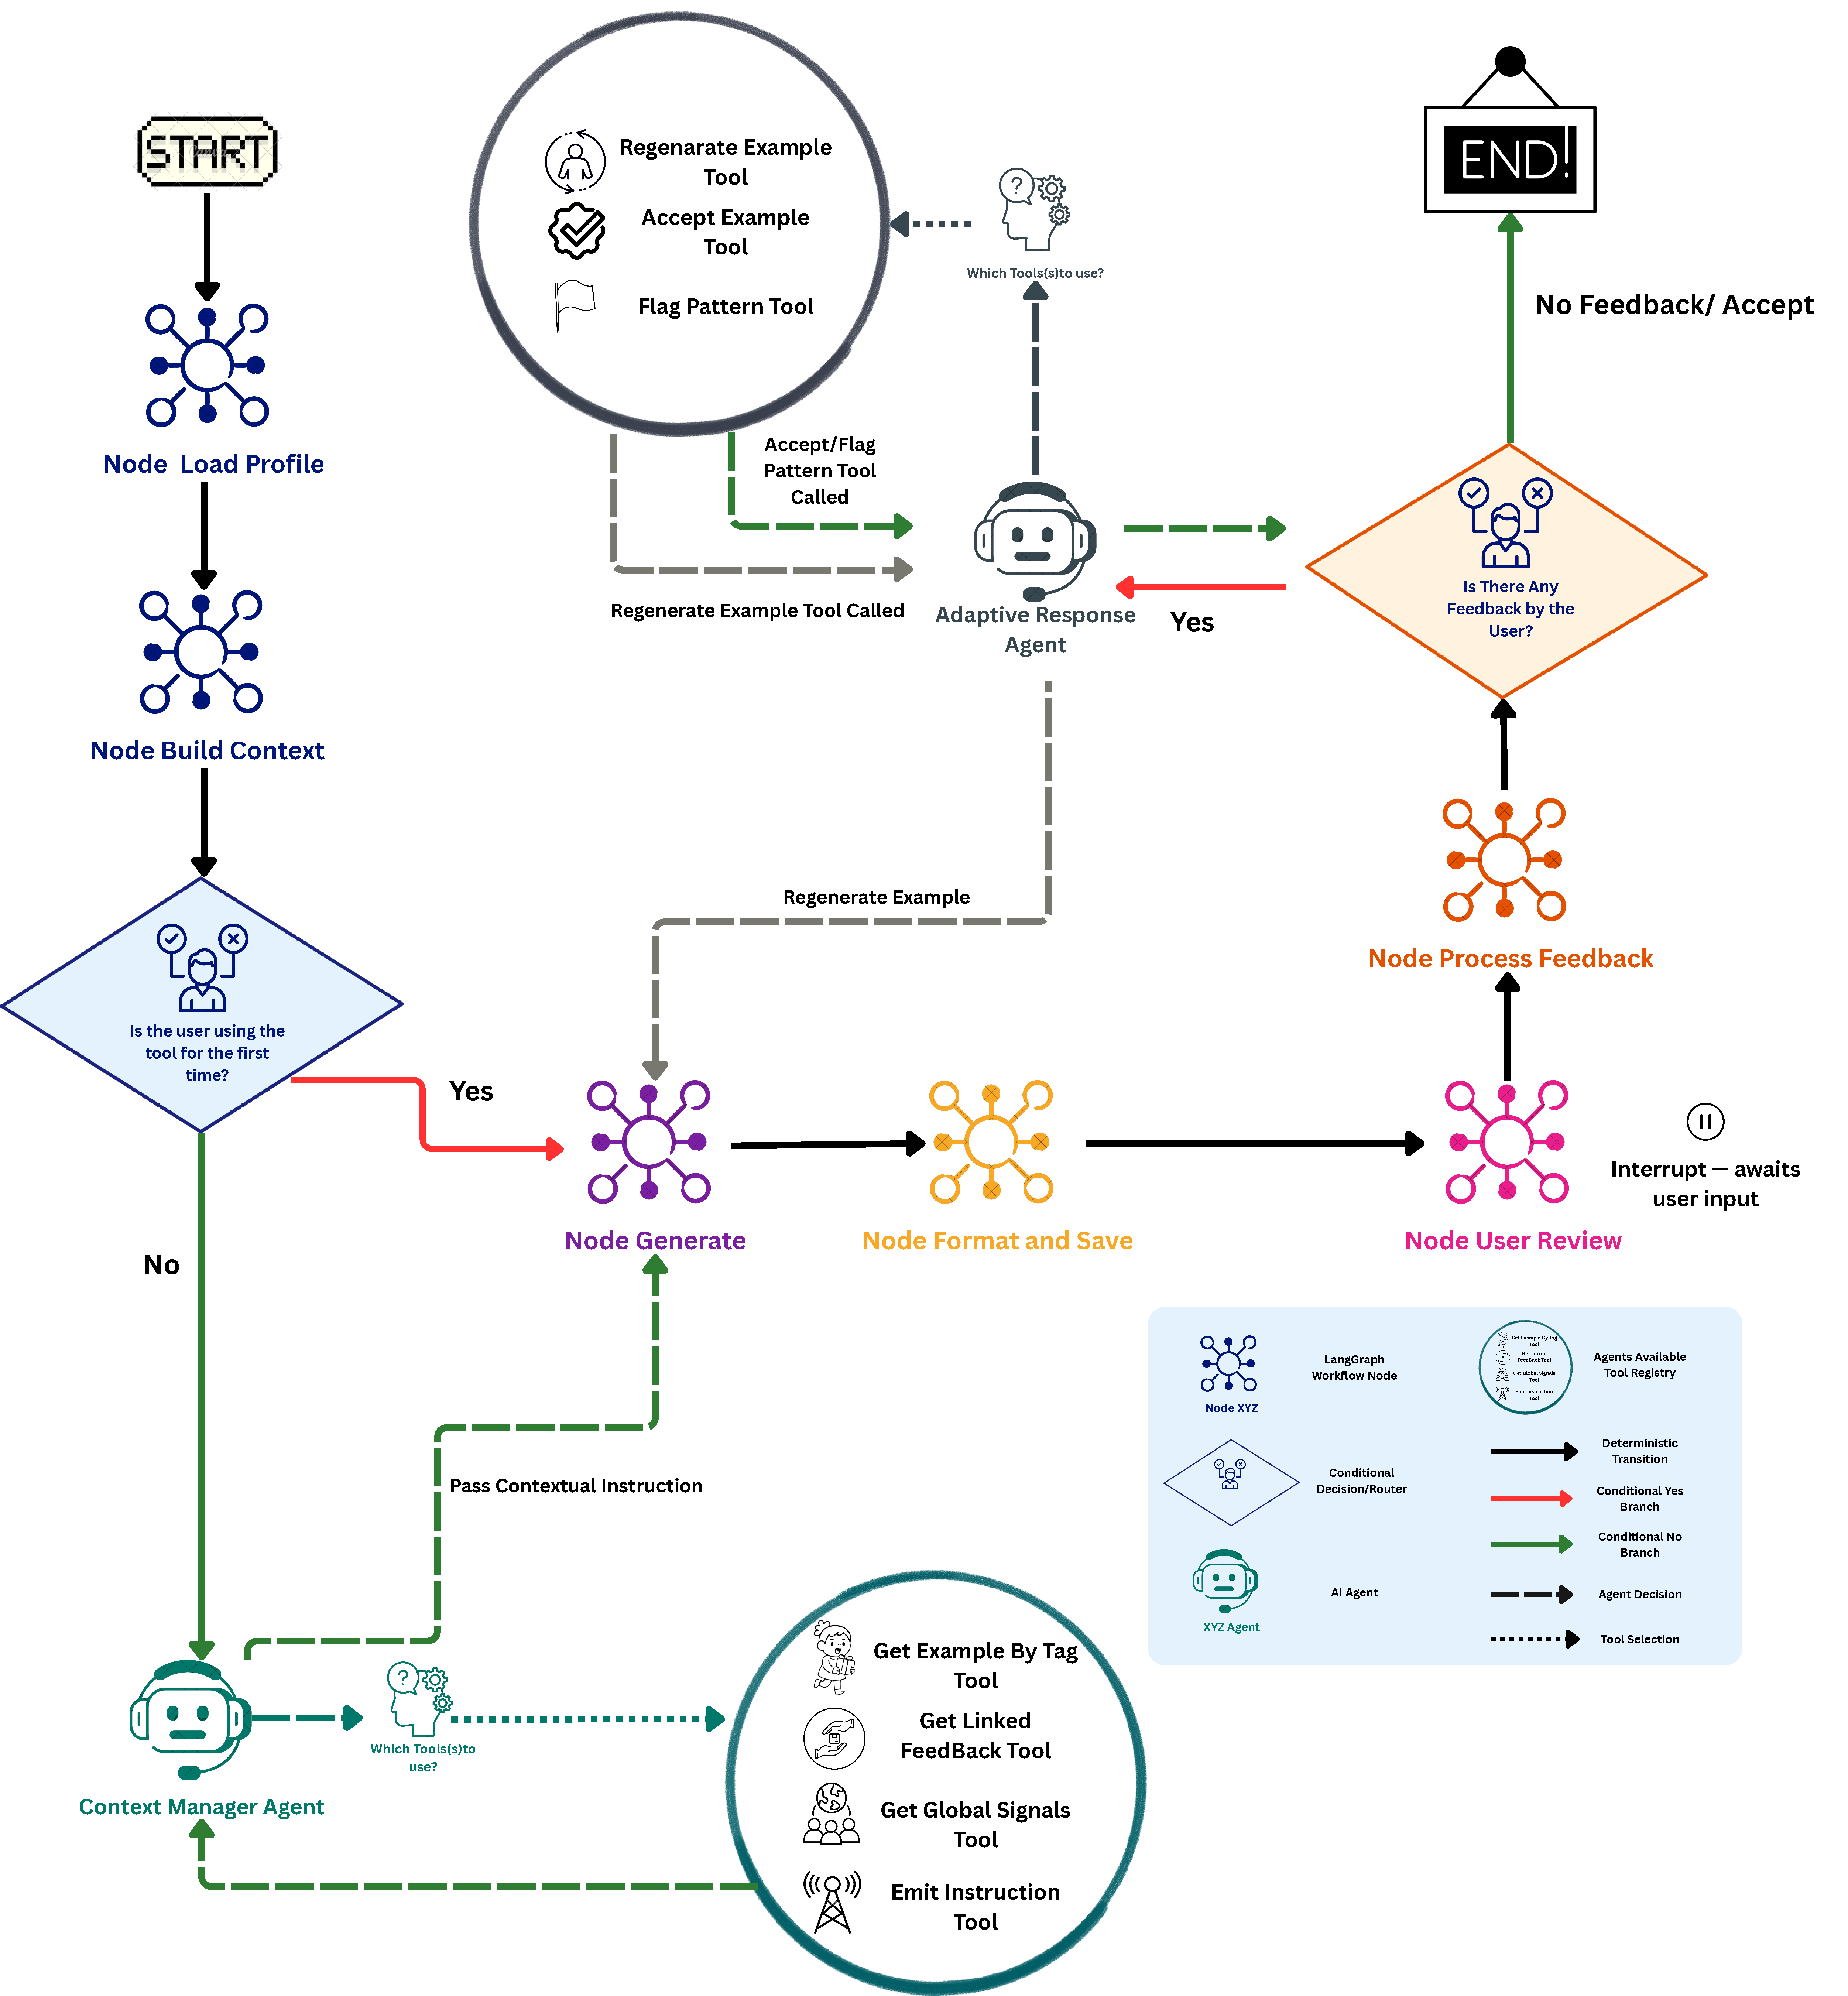
\includegraphics[width=\columnwidth]{workflow.pdf}}
\caption{AdaCraft agentic workflow. Solid black arrows denote deterministic transitions; red/green arrows denote conditional yes/no branches; dashed arrows indicate agent decisions; dotted arrows indicate tool selection. On a returning user's session, the Context Manager Agent (bottom left) selects from four tools (\textit{Get Example By Tag}, \textit{Get Linked Feedback}, \textit{Get Global Signals}, and \textit{Emit Instruction}) to synthesize a personalization instruction passed to the generation node. After the \textbf{Interrupt} at the User Review node (awaiting user input), the Adaptive Response Agent (center) selects from three tools (\textit{Regenerate Example}, \textit{Accept Example}, and \textit{Flag Pattern}), routing the workflow back to generation (up to three cycles) or forward to END.}
\label{fig:workflow}
\end{figure}

\subsection{Node Descriptions}

\textbf{Node Load Profile.} The workflow begins by reading the user's stored profile from persistent JSON storage and converting it into a plain-English summary (e.g., ``Priya is a nurse in Chennai with a simple complexity preference and a visual learning style''). As shown by the solid deterministic arrow from START in Fig.~\ref{fig:workflow}, this node always executes first and its output is threaded through all subsequent LLM calls as the primary personalization signal.

\textbf{Node Build Context and the Context Manager Agent.} As depicted by the conditional router following Node Build Context in Fig.~\ref{fig:workflow}, a first-time user takes the red (yes) branch directly to Node Generate, bypassing the Context Manager Agent entirely. Returning users take the green (no) branch, triggering the agent. Given the current topic, an LLM call first resolves one to three canonical subject tags from a fixed taxonomy (e.g., ``Newton's Second Law'' $\to$ \{physics, mechanics, forces\}). The agent then reasons over the user's history via its tool registry (shown in the bottom-left circle of Fig.~\ref{fig:workflow}), selecting tools via dotted tool-selection arrows. \textit{Get Example By Tag} queries stored examples filtered by each resolved tag, returning recent entries with text snippets and feedback outcomes. \textit{Get Linked Feedback} drills into a specific example to retrieve the learning patterns and accepted insights recorded against it. \textit{Get Global Signals} acts as a fallback when no tag-matched history exists, returning the user's most recent global patterns and insights across all topics. Finally, \textit{Emit Instruction} is called exactly once as the terminal action, writing a two-to-three sentence directive into the workflow state (e.g., ``Use medical equipment analogies. This user struggles with abstract formulas; ground all quantities in clinical measurements''). A domain-bleed guard (a filter that suppresses patterns whose subject tags share no overlap with the current topic's resolved tags) prevents style patterns from prior unrelated sessions from contaminating the instruction; if no relevant signals are found, the agent emits an empty string. The resulting instruction is passed via the dashed agent-decision arrow to Node Generate.

\textbf{Node Generate.} Reached by a deterministic transition from either branch of the first-time router (Fig.~\ref{fig:workflow}), this node composes a combined prompt from three signals: the profile summary, the personalization instruction from the context step, and, in regeneration loops, a targeted rewrite directive carried over from the prior feedback round (cleared from state after use to prevent leakage into further cycles). The system prompt enforces a domain-appropriate structured output format and explicitly prohibits complexity mismatches, domain bleeding (e.g., code snippets in biology examples), and meta-commentary.

\textbf{Node Format and Save.} Connected to Node Generate by a solid deterministic arrow in Fig.~\ref{fig:workflow}, this node records the generated example to the user's example history with its resolved subject tags, a profile snapshot, and session metadata. This enables the Context Manager Agent to retrieve it in future sessions.

\textbf{Node User Review.} As indicated by the interrupt marker in Fig.~\ref{fig:workflow}, LangGraph pauses execution at this node and returns the generated example along with a session token to the caller. The workflow resumes only when the user submits natural-language feedback through the extension.

\textbf{Node Process Feedback and the Adaptive Response Agent.} After the interrupt, a conditional router checks whether the user has provided feedback (Fig.~\ref{fig:workflow}). If there is no feedback or the user accepts the example, the green (no) branch routes directly to END. If feedback is present, the red (yes) branch activates the Adaptive Response Agent. The agent is invoked with four inputs (the feedback text, the example shown, the user profile, and the current pattern history) and selects from three tools shown in the top-left circle of Fig.~\ref{fig:workflow} via dotted tool-selection arrows. When the example needs immediate revision, it calls the \textit{Regenerate Example} tool, which issues a \textbf{regeneration request} with a targeted rewrite directive (e.g., ``Simplify to simple complexity; remove all formulas; use a single concrete scenario from the user's city'') and, as shown by the dashed arrow looping back to Node Generate, routes the workflow back for up to three regeneration cycles. When feedback is positive or neutral, it calls the \textit{Accept Example} tool, recording a session insight for the Context Manager Agent. When feedback reveals a persistent learner trait (a domain preference, recurring difficulty, or stable complexity preference), it calls the \textit{Flag Pattern} tool, persisting a new learning pattern that shapes all future sessions. Both \textit{Accept Example} and \textit{Flag Pattern} route back to the feedback router via the dashed agent-decision arrow, allowing the loop to continue or exit as appropriate.

\subsection{State and Persistence}

The in-session workflow state is a typed dictionary persisted by LangGraph's in-memory checkpointer, keyed by the session token assigned at workflow start. This allows the workflow to pause at the interrupt step and resume seamlessly when the user provides feedback, with all intermediate context, including the profile summary, personalization instruction, and generated example, preserved without recomputation.

Cross-session data is stored in three JSON files per user:
\begin{itemize}
    \item \textbf{Feedback history}: All feedback entries with agent decisions and subject-tag indexes, used for pattern detection and topic-specific signal retrieval.
    \item \textbf{Learning patterns}: Persistent behavioral traits flagged by the Adaptive Response Agent, tagged with pattern type and the example that triggered detection.
    \item \textbf{Accepted insights}: Positive session insights, capped at 50 entries. The cap prevents stale early-session signals from persisting indefinitely while keeping the full list within a single Context Manager prompt without context-window overflow.
\end{itemize}

\section{Evaluation Design}
\label{sec:evaluation}

A central challenge in evaluating AdaCraft is that its value comes not just from the quality of a single example, but from how well the system improves across a feedback loop. Our evaluation design therefore has two parts: a four-tier ablation that isolates each capability layer's individual contribution, and a set of feedback-loop convergence metrics that characterize how the system evolves over multiple rounds.

\subsection{Ablation Structure}

We evaluate AdaCraft via a four-tier ablation grounded in the LaMP benchmark \cite{b3}, where each tier disables exactly one capability layer. This lets us answer three distinct questions: What does knowing the user's profile add? What does the Context Manager Agent add on top of the profile? What does the feedback loop and pattern memory add on top of both? Each tier is implemented via an evaluation-mode flag in the workflow state; three steps perform conditional early-returns based on this flag, requiring no graph rebuilds and ensuring the same codebase services all four conditions.

\begin{table}[htbp]
\caption{Ablation Tiers and Capability Layers}
\label{tab:tiers}
\begin{center}
\begin{tabular}{lccc}
\toprule
\textbf{Tier} & \textbf{Profile} & \textbf{Ctx.Mgr} & \textbf{Feedback \& Patterns} \\
\midrule
T0: Generic LLM   & --  & --  & --  \\
T1: T0+Profile      & \checkmark & --  & --  \\
T2: T1+ContextMgr   & \checkmark & \checkmark & -- \\
T3: Full AdaCraft  & \checkmark & \checkmark & \checkmark \\
\bottomrule
\end{tabular}
\end{center}
\end{table}

The T0$\to$T1 delta isolates the value of profile injection. T1$\to$T2 isolates the Context Manager Agent's contribution. T2$\to$T3 isolates the feedback loop and pattern memory.

\subsection{Evaluation Setup}

\textbf{Synthetic users.} We evaluate across 8 synthetic users, constructed as 4 cultural profiles $\times$ 2 start modes. The four profiles are: a high-school student (Berlin, European), a nurse (Lagos, West African), a humanities researcher (S\~{a}o Paulo, Latin American), and a software engineer (Tokyo, East Asian). This cross-cultural design tests whether the system grounds examples in culturally specific scenarios rather than falling back on generic templates.

\textbf{Topics.} Each user is tested on 4 topics drawn from distinct academic domains (Table~\ref{tab:topics}). The topics were chosen to stress different evaluation axes: psychology and earth sciences target cultural grounding and domain appropriateness; mathematics/finance targets complexity calibration; and evolutionary biology targets conceptual accuracy and pedagogical clarity.

\begin{table}[htbp]
\caption{Evaluation Topics and Primary Axes Tested}
\label{tab:topics}
\begin{center}
\begin{tabular}{lll}
\toprule
\textbf{Domain} & \textbf{Topic} & \textbf{Axis Tested} \\
\midrule
Evolutionary Biology & Natural Selection   & CA, PC \\
Psychology           & Cognitive Bias      & PF, DA \\
Mathematics/Finance  & Compound Interest   & CC, PF \\
Earth Sciences       & Plate Tectonics     & DA, CA \\
\bottomrule
\end{tabular}
\end{center}
\end{table}

\textbf{Cold and warm start.} Users 1--4 begin with no prior interaction history (cold start). Users 5--8 are pre-seeded with 2 learning patterns and 2 accepted insights before evaluation begins (warm start), simulating a returning user with prior sessions. This split enables the PPU metric: for warm-start users, their initial PF scores under T3 (which uses stored patterns via the Context Manager) are compared against their T1 scores (profile only) to quantify how much prior history improves generation.

\textbf{Scripted feedback rounds.} Each T3 session runs three scripted feedback rounds. Four feedback message types are used: a complexity complaint (F1), a domain mismatch complaint (F2), a positive acceptance (F3), and a style preference statement (F4). F1 and F2 are designed to trigger example regeneration; F3 signals that the example was satisfactory; F4 is designed to trigger long-term pattern storage. If a session completes early, for example after an F3 acceptance, a fresh thread is started so that the remaining scripted rounds, including the F4 pattern-flagging round, can still be exercised. Sessions under T0--T2 run only one feedback round, since the Adaptive Response Agent is not active in those tiers.

\textbf{Scale.} Each run covers $8 \times 4 = 32$ (user, topic) pairs per tier, across 4 tiers, giving 128 evaluation cells per generator run. The full study spans 256 cells across two generator configurations (DeepSeek V3.2 and GPT-5-nano).

\subsection{Five-Axis Evaluation Rubric}

Each example is scored 1--5 on five axes by an LLM judge using G-Eval chain-of-thought \cite{b4} (the judge reasons step by step before assigning a score) and Prometheus~2 rubric injection \cite{b5} (the full rubric definition is included in every judge prompt). Weights reflect a pedagogical priority ordering set before any data was collected, yielding the composite score in Eq.~\ref{eq:composite}.

\begin{equation}
C = 0.20 \cdot \text{PF} + 0.20 \cdot \text{CC} + 0.30 \cdot \text{CA} + 0.20 \cdot \text{PC} + 0.10 \cdot \text{DA}
\label{eq:composite}
\end{equation}

\begin{itemize}
    \item \textbf{Personalization Fidelity (PF, 0.20):} Does the example reflect the user's cultural background, occupation, and domain? Grounded in profile-conditioned generation benchmarks \cite{b3, b8}.
    \item \textbf{Complexity Calibration (CC, 0.20):} Does the example's depth and vocabulary match the user's requested complexity level? Motivated by learner-appropriate content design \cite{b13}.
    \item \textbf{Conceptual Accuracy (CA, 0.30):} Is the example factually and logically correct? Weighted highest because no degree of personalization can redeem a misconception \cite{b14}.
    \item \textbf{Pedagogical Clarity (PC, 0.20):} Is the concept explained in a clear, structured, and learner-friendly way? Drawn from educational content quality frameworks \cite{b4, b13}.
    \item \textbf{Domain Appropriateness (DA, 0.10):} Does the example stay within the user's domain without inappropriate cross-domain elements? Weighted lowest as it largely follows from PF and CC in practice \cite{b13}.
\end{itemize}


\subsection{LLM Judge Design}

We use GPT-4.1-nano as the primary evaluation judge across both generator runs. \textbf{Run~1} uses DeepSeek V3.2 \cite{b15} as the generator; \textbf{Run~2} uses GPT-5-nano \cite{b16}. Keeping the judge fixed while varying the generator provides cross-provider evaluation independence and specifically mitigates self-enhancement bias \cite{b11}, where a model tends to score outputs resembling its own generation style more favorably, a concern noted for Run~2, where judge and generator share the same provider family. GPT-4.1-nano is cost-efficient at the scale of 256 evaluation cells (128 per run) while maintaining strong rubric-following capability. A secondary judge (Llama~3.3~70B) was deployed on a 20\% random subsample for inter-judge agreement verification (Cohen's~$\kappa$).

Two additional bias mitigations are applied:
\begin{itemize}

    \item \textit{Verbosity bias:} the judge system prompt explicitly instructs the model to penalize length and reward conciseness and clarity.
    \item \textit{Self-enhancement:} T0 generic examples are evaluated with separate judge invocations, not in direct comparison with profile-aware outputs, to prevent anchoring effects.
\end{itemize}

\subsection{Feedback Loop Convergence Metrics}

Standard quality rubrics measure a snapshot. For T3, we additionally compute three metrics that characterize the quality of the feedback loop itself over time. These metrics are designed to be applicable to any LLM system with a human-in-the-loop refinement process, not just AdaCraft.

\begin{itemize}
    \item \textbf{FCR (Feedback Compliance Rate):} The fraction of regenerations that correctly address the prior critique, as determined by the judge's compliance scoring. A regeneration is ``compliant'' if the judge assigns a compliance score $\geq 3$ on a 1--5 scale, the Likert midpoint, interpreted as ``the main substance of the critique was addressed even if imperfectly.'' We additionally report FCR@4 (score $\geq 4$) as a stricter quality threshold so that both an adequacy bar and a quality bar are visible and neither can be cherry-picked.
    \item \textbf{LUR (Loop Utilization Rate):} The fraction of T3 sessions where the Adaptive Response Agent triggered at least one regeneration in response to a complaint message. An LUR of 1.0 means the agent correctly identified every scripted complaint as requiring a revision, with no false negatives.
    \item \textbf{PPU (Pattern Persistence Utilization):} In short: do returning users with stored learning patterns get better first-generation examples than returning users without them? Formally, PPU is the mean PF score delta between warm-start T3 sessions (profile + Context Manager + seeded patterns) and warm-start T1 sessions (profile only, same users, same topics) on the \textit{initial} generated example, before any feedback is given. A positive delta indicates that the Context Manager Agent's retrieval and synthesis of stored patterns produces measurably better personalization than the static profile alone. Cold-start T3 sessions serve as a secondary control: if warm T3 PF $>$ cold T3 PF, the difference is attributable to the seeded patterns rather than to the Context Manager architecture itself.
\end{itemize}

\section{Results and Discussion}
\label{sec:results}

We report results from two generator configurations evaluated on the same 128-cell grid (8 users $\times$ 4 topics $\times$ 4 tiers), judged by GPT-4.1-nano throughout. Run~1 uses DeepSeek V3.2 \cite{b15}; Run~2 uses GPT-5-nano \cite{b16}. Evaluating both generators with an identical harness and fixed judge isolates generator-specific effects from evaluation-framework effects.

\subsection{Ablation Results}

Table~\ref{tab:ablation_results} reports mean composite and per-axis scores for each tier across both runs, showing clear monotonic improvement across all capability layers in both generator configurations.

\begin{table}[htbp]
\caption{Ablation Results: Mean Scores by Tier (DS=DeepSeek V3.2, G5=GPT-5-nano)}
\label{tab:ablation_results}
\begin{center}
\scriptsize
\setlength{\tabcolsep}{6pt}
\begin{tabular}{llccccccc}
\toprule
\textbf{Run} & \textbf{Tier} & \textbf{PF} & \textbf{CC} & \textbf{CA} & \textbf{PC} & \textbf{DA} & \textbf{Comp.} & \textbf{$\Delta$T0} \\
\midrule
\multirow{4}{*}{DS}
 & T0 & 2.73 & 4.13 & 4.94 & 4.82 & 4.39 & 4.257 & --- \\
 & T1 & 4.80 & 4.35 & 4.99 & 4.93 & 4.95 & 4.809 & +0.552 \\
 & T2 & 4.93 & 4.43 & 5.00 & 4.95 & 4.99 & 4.859 & +0.602 \\
 & T3 & 4.99 & 4.47 & 5.00 & 4.99 & 5.00 & 4.888 & +0.631 \\
\midrule
\multirow{4}{*}{G5}
 & T0 & 2.09 & 3.78 & 4.41 & 4.00 & 4.16 & 3.712 & --- \\
 & T1 & 3.47 & 4.38 & 4.78 & 4.53 & 4.78 & 4.388 & +0.676 \\
 & T2 & 4.34 & 4.84 & 4.97 & 4.88 & 4.88 & 4.791 & +1.079 \\
 & T3 & 4.94 & 5.00 & 5.00 & 4.97 & 5.00 & 4.981 & +1.269 \\
\bottomrule
\end{tabular}
\end{center}
\end{table}

\subsection{DeepSeek V3.2 Results}

DeepSeek V3.2 shows consistent, monotonic improvement across all four tiers. The largest single gain is at T0$\to$T1 ($+0.552$ composite), where profile injection lifts PF from 2.73 to 4.80, a 76\% increase, confirming that knowing who the learner is dominates all other personalization signals. DeepSeek maintains high CA throughout, with baseline CA = 4.94 at T0 and reaching CA $\approx$ 5.00 at T1--T3, demonstrating strong factual grounding even without personalization context. The Context Manager (T1$\to$T2) contributes $+0.050$ and the full feedback loop (T2$\to$T3) contributes a further $+0.029$, bringing the total T0$\to$T3 gain to $+0.631$. The pattern shows that profile injection dominates the improvement curve, with agentic layers providing smaller but consistent incremental gains.

\subsection{GPT-5-nano Results}

GPT-5-nano starts from a weaker baseline than DeepSeek, with a T0 composite of 3.712 compared to DeepSeek's 4.257, and CA = 4.41 at T0 compared to DeepSeek's 4.94, indicating that without profile context, GPT-5-nano's factual grounding and overall content quality are less robust. However, GPT-5-nano responds more strongly to each successive capability layer. The T1$\to$T2 gain ($+0.403$) substantially exceeds the corresponding DeepSeek delta, while the T2$\to$T3 gain ($+0.190$) reflects convergence near ceiling. T3 reaches a composite of 4.981 with all five axes at or near maximum. The total T0$\to$T3 gain is $+1.269$, the largest overall lift in the study, indicating that GPT-5-nano benefits significantly more from agentic layering than DeepSeek. This pattern suggests GPT-5-nano is more responsive to structured context and feedback instructions, but requires those signals to achieve high reliability.

\subsection{Cross-Provider Analysis}

Both generators produce a strict monotonic ordering T0 $<$ T1 $<$ T2 $<$ T3. The T0$\to$T1 delta is the largest single-tier gain in both runs, establishing profile injection as the dominant driver of personalization quality regardless of generator. The agentic layers (T1$\to$T2 and T2$\to$T3) provide compounding but smaller increments, confirming that they add genuine value beyond the profile baseline without outweighing it.

Inter-judge agreement between GPT-4.1-nano and the Llama~3.3~70B secondary judge, evaluated on a 20\% random subsample, yielded Cohen's $\kappa$ = \textbf{0.607} for the DeepSeek run and $\kappa$ = \textbf{0.681} for the GPT-5-nano run, both indicating moderate to substantial agreement and supporting the reliability of GPT-4.1-nano as a standalone judge at full evaluation scale.

\subsection{Feedback Loop Convergence (T3)}

Table~\ref{tab:convergence} reports the three convergence metrics for T3 sessions, which provide a more direct window into how the agentic feedback loop operates.

\begin{table}[htbp]
\caption{T3 Feedback Loop Convergence Metrics (DS=DeepSeek V3.2, G5=GPT-5-nano)}
\label{tab:convergence}
\begin{center}
\scriptsize
\setlength{\tabcolsep}{6pt}
\begin{tabular}{llccc}
\toprule
\textbf{Metric} & \textbf{Description} & \textbf{DS} & \textbf{G5} & \textbf{Target} \\
\midrule
FCR@3 & Compliance $\geq 3/5$ & 1.000 & 0.945 & $\geq 0.75$ \\
FCR@4 & Compliance $\geq 4/5$ & 0.902 & 0.891 & $\geq 0.75$ \\
LUR   & Loop Utilization     & 0.938 & 0.969 & $\approx 1.0$ \\
PPU Delta PF & Warm T3 $-$ T1 PF & $+0.312$ & $+1.938$ & $> 0$ \\
\bottomrule
\end{tabular}
\end{center}
\end{table}

\textbf{FCR.} For DeepSeek V3.2: FCR@3 = 1.000 and FCR@4 = 0.902 (41 regenerations; mean compliance 4.34/5). For GPT-5-nano: FCR@3 = 0.945 and FCR@4 = 0.891 (55 regenerations; mean compliance 4.56/5). Both runs exceed the $\geq 0.75$ adequacy target by a wide margin. Breaking down by feedback type: DeepSeek achieves FCR@4 = 1.000 on easy feedback (28 regenerations) but 0.692 on adversarial feedback (13 regenerations), which pulls its overall FCR@4 to 0.902. GPT-5-nano achieves FCR@4 = 0.850 on easy feedback (40 regenerations) and 1.000 on adversarial (15 regenerations), with lower easy-feedback compliance accounting for its overall FCR@4 of 0.891. The directional finding holds across both providers: the agent reliably translates natural-language critiques into targeted regenerations for clear, specific feedback types, consistent with the iterative refinement paradigm of Self-Refine \cite{b12}.

\textbf{LUR.} DeepSeek: LUR = 0.938 (30/32 sessions triggered at least one regeneration). GPT-5-nano: LUR = 0.969 (31/32). Both approach the $\approx 1.0$ target, confirming the Adaptive Response Agent correctly identifies scripted F1/F2 complaint messages with high reliability. Missed triggers in each run reflect feedback phrasing that was ambiguous enough to be classified as neutral rather than regeneration-warranting.

\textbf{PPU.} DeepSeek: $\Delta$PF = $+0.312$ (warm T3 initial PF = 5.00 vs.\ warm T1 PF = 4.688; cold T3 PF = 4.979, $n = 16$ per group). GPT-5-nano: $\Delta$PF = $+1.938$ (warm T3 PF = 5.00 vs.\ warm T1 PF = 3.062; cold T3 PF = 5.000). In both runs, warm-start T3 sessions score higher on initial PF than warm-start T1 sessions (same users, same topics), confirming that stored learning patterns provide a meaningful personalization increment at first generation. For DeepSeek, the modest delta reflects that profile injection alone already achieves high personalization (PF $\approx$ 4.7--5.0), with patterns providing incremental gains. For GPT-5-nano, the larger delta (6.2x greater than DeepSeek) reflects its substantially lower baseline personalization (T1 PF = 3.062 vs DeepSeek T1 PF = 4.688), where patterns have significantly more room to improve initial examples, demonstrating differential value across generator types.


\section{Limitations and Future Work}

\textbf{Synthetic user study.} The 8 evaluation users are constructed, not real learners. Although the profiles span four distinct cultural and professional backgrounds, actual users may reveal failure modes that scripted feedback cannot capture: for example, ambiguous feedback that the agent misinterprets, mid-session topic drift, or multi-issue feedback (e.g., ``make it simpler and use a different domain'') that the agent must decompose rather than act on as a single signal. A user study with real learners is planned as future work.

\textbf{Single-session pattern seeding.} The warm-start protocol seeds two patterns per user from a fixed template. Real pattern accumulation over many sessions may produce richer, more specific context instructions. A longitudinal study over at least 5 sessions per user would better characterize long-term PPU behavior.

\section{Conclusion}

AdaCraft shows that iterative, feedback-driven personalization is both architecturally feasible and measurably better than static profile injection. Across two generator configurations, DeepSeek V3.2 and GPT-5-nano, each capability layer adds a consistent, independent increment to personalization quality, with the full system (T3) outperforming a generic baseline by up to $+1.269$ composite points. The agentic feedback loop proves reliable in both runs: the Adaptive Response Agent correctly acts on user complaints at FCR@4 $\geq 0.891$ across both providers and regenerates in at least 93\% of sessions (LUR), and stored learning patterns measurably improve first-generation quality for returning users, with PPU deltas ranging from +0.312 (DeepSeek, already high-baseline) to +1.938 (GPT-5-nano, showing pattern impact at lower baseline). The four-tier ablation design and the FCR, LUR, and PPU metrics together offer a reusable evaluation framework for any LLM system that combines profile-grounded generation with iterative human-in-the-loop refinement, a paradigm that static personalization benchmarks are not designed to capture.

% Acknowledgment removed for blind review


\begin{thebibliography}{00}

\bibitem{b1}
Z. Zhang, R. A. Rossi, B. Kveton, Y. Shao, D. Yang, H. Zamani, F. Dernoncourt, J. Barrow, T. Yu, S. Kim, R. Zhang, J. Gu, T. Derr, H. Chen, J. Wu, X. Chen, Z. Wang, S. Mitra, N. Lipka, N. Ahmed, and Y. Wang, ``Personalization of Large Language Models: A Survey,'' \textit{arXiv preprint arXiv:2411.00027}, 2024.

\bibitem{b2}
J. Liu, Z. Qiu, Z. Li, Q. Dai, W. Yu, J. Zhu, M. Hu, M. Yang, T.-S. Chua, and I. King, ``A Survey of Personalized Large Language Models: Progress and Future Directions,'' \textit{arXiv preprint arXiv:2502.11528}, 2025.

\bibitem{b3}
A. Salemi, S. Mysore, M. Bendersky, and H. Zamani, ``LaMP: When Large Language Models Meet Personalization,'' in \textit{Proc. 62nd Annu. Meeting Assoc. Comput. Linguistics (ACL)}, Bangkok, Thailand, 2024, pp. 7370--7392.

\bibitem{b4}
Y. Liu, D. Iter, Y. Xu, S. Wang, R. Xu, and C. Zhu, ``G-Eval: NLG Evaluation Using GPT-4 with Better Human Alignment,'' in \textit{Proc. 2023 Conf. Empirical Methods Nat. Lang. Process. (EMNLP)}, 2023, pp. 2511--2522.

\bibitem{b5}
S. Kim, J. Suk, S. Longpre, B. Y. Lin, J. Shin, S. Welleck, G. Neubig, M. Lee, K. Lee, and M. Seo, ``Prometheus 2: An Open Source Language Model Specialized in Evaluating Other Language Models,'' in \textit{Proc. 2024 Conf. Empirical Methods Nat. Lang. Process. (EMNLP)}, 2024, pp. 4334--4353.

\bibitem{b6}
J. Sweller, ``Cognitive Load During Problem Solving: Effects on Learning,'' \textit{Cognitive Science}, vol. 12, no. 2, pp. 257--285, 1988.

\bibitem{b7}
J. Hattie and H. Timperley, ``The Power of Feedback,'' \textit{Rev. Educ. Res.}, vol. 77, no. 1, pp. 81--112, 2007.

\bibitem{b8}
I. Kumar, S. Viswanathan, S. Yerra, A. Salemi, R. A. Rossi, F. Dernoncourt, H. Deilamsalehy, X. Chen, R. Zhang, S. Agarwal, N. Lipka, C. V. Nguyen, T. H. Nguyen, and H. Zamani, ``LongLaMP: A Benchmark for Personalized Long-form Text Generation,'' \textit{arXiv preprint arXiv:2407.11016}, 2024.

\bibitem{b9}
LangChain~Inc., ``LangGraph: Build Resilient Language Agents as Graphs,'' 2024. [Online]. Available: \url{https://github.com/langchain-ai/langgraph}. [Accessed: Mar.~26, 2026].

\bibitem{b10}
B. Jiang, Z. Hao, Y.-M. Cho, B. Li, Y. Yuan, S. Chen, L. Ungar, C. J. Taylor, and D. Roth, ``Know Me, Respond to Me: Benchmarking LLMs for Dynamic User Profiling and Personalized Responses at Scale,'' in \textit{Proc. 2nd Conf. Lang. Modeling (COLM)}, 2025.

\bibitem{b11}
L. Zheng, W.-L. Chiang, Y. Sheng, S. Zhuang, Z. Wu, Y. Zhuang, Z. Lin, Z. Li, D. Li, E. P. Xing, H. Zhang, J. E. Gonzalez, and I. Stoica, ``Judging LLM-as-a-Judge with MT-Bench and Chatbot Arena,'' in \textit{Adv. Neural Inf. Process. Syst. (NeurIPS)}, vol. 36, 2023.

\bibitem{b12}
A. Madaan, N. Tandon, P. Gupta, S. Hallinan, L. Gao, S. Wiegreffe, U. Alon, N. Dziri, S. Prabhumoye, Y. Yang, S. Gupta, B. P. Majumder, K. Hermann, S. Welleck, A. Yazdanbakhsh, and P. Clark, ``Self-Refine: Iterative Refinement with Self-Feedback,'' in \textit{Adv. Neural Inf. Process. Syst. (NeurIPS)}, vol. 36, 2023.

\bibitem{b13}
K. K. Maurya, K. V. A. Srivatsa, K. Petukhova, and E. Kochmar, ``Unifying AI Tutor Evaluation: An Evaluation Taxonomy for Pedagogical Ability Assessment of LLM-Powered AI Tutors,'' in \textit{Proc. 2025 Conf. Nations Americas Chapter Assoc. Comput. Linguistics: Human Lang. Technol. (NAACL)}, 2025, pp. 1234--1251.

\bibitem{b14}
W. Feng, J. Lee, H. McNichols, A. Scarlatos, D. Smith, S. Woodhead, N. Ornelas, and A. Lan, ``Exploring Automated Distractor Generation for Math Multiple-Choice Questions via Large Language Models,'' in \textit{Findings Assoc. Comput. Linguistics: NAACL 2024}, Mexico City, Mexico, 2024, pp. 3067--3082.

\bibitem{b15}
DeepSeek-AI, ``DeepSeek-V3 Technical Report,'' \textit{arXiv preprint arXiv:2412.19437}, 2024.

\bibitem{b16}
OpenAI, ``Introducing GPT-4.1 in the API,'' OpenAI, Apr.~14, 2025. [Online]. Available: \url{https://openai.com/index/gpt-4-1/}. [Accessed: Mar.~26, 2026].

\end{thebibliography}

\end{document}
